\chapter{Fundamentos de máquinas y motores térmicos}
\section{Definiciones}
\paragraph{Máquina de fluido.} Conjunto de elementos mecánicos que permiten intercambiar energía mecánica con el exterior a través de un eje mediante la variación de energía del fluido que atravisa la máquina. Pueden ser de dos tipos:
\begin{itemize}
    \item Máquinas Hidráulicas. Utilizan fluido incompresible, es decir un líquido o un gas que puede tratarse como incompresible cuando la variación de densidad es muy pequeña a su paso por la máquina. Ej.: turbinas y bombas hidráulicas, ventiladores y aerogeneradores.
    \item Máquinas Térmicas. Utilizan un fluido compresible, es decir en el que la variación de densidad o volumen específico es significativo a su paso por la máquina y forma parte del intercambio energético. Ej.: Turbinas de vapor y gas, compresores y motores alternativos.
\end{itemize}

\paragraph{Máquina Térmica.} Maquina de fluido compresible que intercambia energía mecánica con el exterior a través de la variación de la energía térmica de un fluido que la atravisa.

\paragraph{Motor Térmico.} Conjunto de elementos mecáncos que permiten obtener energía mecánica, generalmente a través de un eje, mediante el estado térmico generado en una reacción de combustión, una reacción nuclear, concentración de radiación solar o, de forma general, un intercambiador de calor.

\section{Cuadro de las transformaciones energéticas}
Todas las formas de energías que hay pueden organizarse en un cuadro de las energías como el de la figura \ref{fig: cuadro de transformaciones energeticas}. El concepto de estado térmico implica la existencia de un fluido a alta temperatura, pero para que pueda dar trabajo en una máquina térmica motora necesita que el fluido tenga una presión mayor que en la descarga. El estado térmico puede transferirse en forma de calor de un fluido a otro.

\begin{figure}[h]
    \centering
    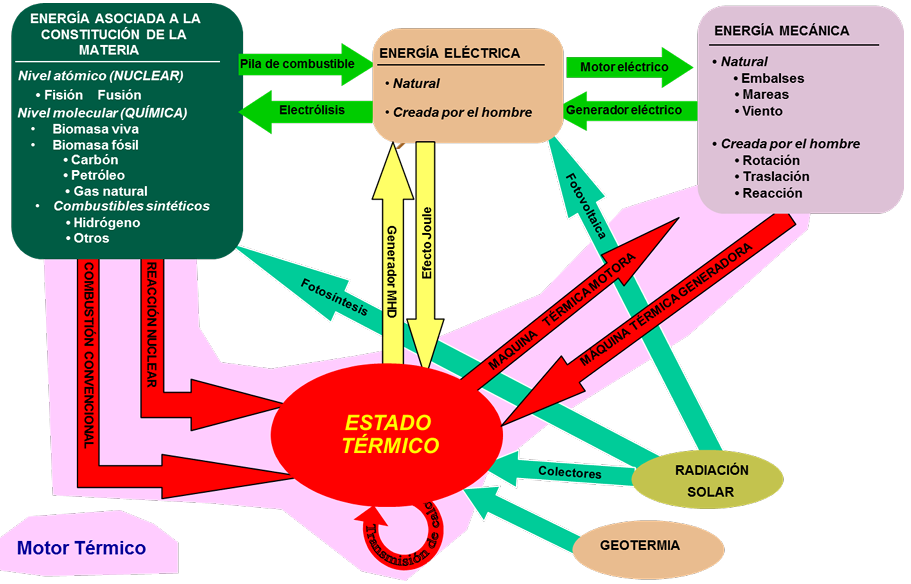
\includegraphics[width = \linewidth]{Imagenes/Cuadro de las transformaciones energeticas.png}
    \caption{Cuadro de las Energías}
    \label{fig: cuadro de transformaciones energeticas}
\end{figure}

Las transformaciones energéticas marcadas en rojo en la figura \ref{fig: cuadro de transformaciones energeticas} conforman lo que es un motor térmico. El estado térmico se genera por medio de una máquina térmica generadora y a partir de energía asociada a la constitución de la materia por medio de una reacción de combustión o nuclear. Normalmente se usan ambos métodos. La máquina térmica motora es la encargada de transformar el estado térmico en trabajo mecánico.

\section{Clasificaación de las máquinas térmicas}
Las máquinas térmicas se clasifican dentro de dos categorías. Por un lado, se clasifican en función del sentido de la energía:
\begin{itemize}
    \item Máquinas Motoras o Expansores: son aquellas en las que la energía del fluido disminuye produciendo trabajo mecánico.
    \item Máquinas Generadoras o Compresores: son aquellas en las que la energía del fluido aumenta, para lo cual hace falta aportar trabajo mecánico desde el exterior.
\end{itemize}

A su vez, las máquinas térmicas pueden ser de dos tipos:
\begin{itemize}
    \item Máquinas Volumétricas: son aquellas en las que la variación de entalpía del fluido se basa en la variación de un volumen geométrico en el interior del cual está conflinado el fluido compresible. Por tanto, el proceso es secuencial y no continua y periódicamente deben descargar o cargar de nuevo. A su vez pueden ser de dos tipo:
    \begin{itemize}
        \item Alternativas: el volumen en el que se confina el gas es un cilindro con émbolo o pistón desplazándose linealmente.
        \item Rotativas: existe un volumen de gas confinado que varía secuencialmente pero el movimiento principal del émbolo es rotativo.
    \end{itemize}
    \item Máquinas Dinámicas o Turbomáquinas: son aquellas en las que el fluido aumenta o reduce su presión mediante procesos fluiddinámicos basados en su paso por conductos de sección variable en coronas móviles y fijas. Por su esencia son siempre rotativas y el flujo es continuo. Cuando son motoras se denominan turbinas y cuando son generadoras se denomminan turbocompresores.
\end{itemize}

\section{Clasificación de los motores térmicos}
Los motores térmicos se clasifican atendiendo al modo de realizar la generación del estado térmico en tres grandes grupos:
\begin{itemize}
    \item Según la renovación del flido de trabajo:
    \begin{itemize}
        \item Motores de Ciclo Cerrado. El fluido de trabajo realiza el ciclo termodinámico de manera cícloca, sin ser renovado. La cesión de calor se realiza a través de un intercambiador de calor con el ambiente, lo que obliga a que la variable atmosférica que condiciona el ciclo sea la temperatura de ambiente; es decir, la temperatura mínima del ciclo no podrá ser inferior a esta. Finalmente, los motores de ciclo cerrado solo pueden ser aplicables en caso de motores de combustión externa.
        \item Motores de Ciclo Abierto. El fluido de trabajo se renueva de manera continua no circulando de manera cíclica a través del motor. La cesión de calor no se realiza a través de un intercambiador de calor, sino a través del enfriamiento del fluido tras su escape al ambiente y la admisión de fluido que no ha circulado previamente. Al realizar el escape al ambiente, la variable atmosférica que condicionará el ciclo será la presión atmosférica, pues la presión del ciclo en el escape debe coincidir con ella. Son solo usados cuando el fluido de trabajo es aire o, en casos excepcionales, cuando el fluido de trabajo tiene coste nulo o despreciable. Finalmente, en la inmensa mayoría de los casos, los motores de ciclo abierto se usan en el caso de motores de combustión interna.
    \end{itemize}
    \item Según el lugar de la generación del estado térmico:
    \begin{itemize}
        \item Motores de Combustión Externa. En ellos la combustión, reacción nuclear u otro método de generación de estado térmico ocurre en un fluido diferente al fluido de trabajo que es el que participa en la producción de trabajo mecánico en la máquina térmica motora. Por tanto existe un proceso de transferencia de calor entre el estado térmico y el fluido de trabajo. En este caso, el motor recibe calor del foco caliente ($\dot{Q}_{FC}$) proveniente de una combustión, una reacción nuclear, del sol, etc.; y cede calor al foco frío ($\dot{Q}_{FF}$) que es el medio ambiente, además de dar potencia útil. El rendimiento de estos motores se define como:
        \begin{equation}
            \eta_t = \frac{\dot{W}_u}{\dot{Q}_{FC}} = \frac{\dot{W}_u}{\dot{W}_u + \dot{Q}_{FF}}
        \end{equation}
        Estos motores son normalmente de ciclo cerrado, pues el fluido de trabajo una vez expandido puede recuperarse para recibir de nuevo el estado térmico y volver a producir trabajo en la máquina motora al no sufrir transformaciones química.
        \item Motores de Combustión Interna. En esos el proceso de combustión ocurre en el mismo fluido de trabajo, por lo tanto, no es necesario el proceso de transferencia de calor y en la máquina térmica motora se expanden los gases provenientes de la combustión. En estos motores entra aire y combustible ($\dot{m}_a$ y $\dot{m}_f$) a temperatura del medio ambiente y el combustible tiene una energía química basada en sus entalpías de formación de sus componentes, que es su poder calorífico. Normalmente se utiliza el poder calorífico inferior (PCI) o entalpía de combustión ($H_c$). Como energías salientes están la potencia útil ($\dot{W}_u$), la energía térmica por pérdidas de calor ($\dot{Q}$) y la energía de los gases de escape, que está a su vez compuesta por la suma de la energía térmica y la energía química de los posibles productos de combustión incompleta.
        \begin{equation}
            \eta_t = \frac{\dot{W}_u}{\dot{m}_f \cdot H_c}
        \end{equation}
        Estos motores son necesariamente de ciclo abierto, pues no pueden reutilizar los gases de la combustión para realizar de nuevo otra combustión.
    \end{itemize}
    \item Según la forma de obtener la potencia:
    \begin{itemize}
        \item Motores de Potencia en un Eje Rotativo. El eje transmite par motor al elemento accionado. La potencia obtenida por el motor es el producto del par transmitido por la velocidad angular del eje:
        \begin{equation}
            \dot{W}_e = M \cdot \omega
        \end{equation}
        Estos motores pueden accionar máquinas o sistemas de propulsión. A su vez, se clasifican en motores alternativos (volumétricos) y motores de flujo continuo basados en turbomáquinas.
        \begin{itemize}
            \item Motores Volumétricos (alternativos). Se basan en máquinas volumétricas
        \end{itemize}
        \item Motores de Reacción.
    \end{itemize}
\end{itemize}

\section{Campos de aplicación de los motores térmicos}

\section{Ciclo combinado y cogeneración}

\section{Conceptos de combustión y emisiones contaminantes}